\chapter{Perfcake}\label{perfcake}
\setcounter{page}{1}
\pagenumbering{arabic}

Táto kapitola sa venuje nástroju na testovanie výkonu Perfcake, jeho použitiu a typu dát, ktoré generuje. 

\begin{figure}[ht]

\includegraphics[scale=1]{blog-logo.png}
\caption{Perfcake}
\end{figure} 

\section{O nástroji}

Perfcake je open-source framework vyvíjaný spoločnosťou Red Hat. Ako sa píše na oficiálnej stránke tohto nástroja, je to generátor zaťaženia s cieľom byť minimalistický a ľahko ovládateľný, poskytujúci stabilné výsledky, majúci minimálny vplyv na testovaný systém, byť nezávislý na platforme, umožňujúci vysokú priepustnosť a používajúci komponentový dizajn.

Perfcake vie vytvoriť niekoľko možností zaťaženia, môže:
\begin{itemize}  
\item vytvoriť prednastavený počet správ,
\item poslať toľko správ koľko je testovaný softvér schopný za určitú časovú jednotku spracovať,
\item sa opatrne pokúsiť o maximálny možný výkon testovaného softvéru.
\end{itemize}

Užívateľ má niekoľko možností reportovania výsledkov, ako napríklad výpis na konzolu, súbor logov alebo tiež CSV formát. Nástroj tiež poskytuje viac možností výsledkov, vrátane priemernej priepustnosti alebo veľkosti spotrebovanej pamäte cieľovej JVM (Java virtual machine), s možnosťou regresnej analýzy za účelom odhalenia úniku pamäte.

Jeden z problémov podobných testovacích nástrojov je prípad, kedy testovaný softvér zlyhá a vzápätí odošle chybovú správu. Pre tento prípad sú v nástroji Perfcake zabudované validátory, ktoré dokážu takúto správu rozpoznať a nezaviesť tým chybové správy do výsledku výkonu softvéru. Podobné softvéry, ktoré takéto validácie neprevádzajú potom vytvárajú veľmi skreslený výsledok.

\section{Použitie}

Pre spustenie nástroja Perfcake je potrebné vytvoriť XML (eXtensible Markup Language) súbory, takzvané scenáre (scenarios). V týchto súboroch sú definované testovacie bloky, ktoré obsahujú cieľový softvér, typ zaťaženia, typ výstupu, typ protokolu, dobu trvania\dots

Validátory sa konfigurujú spolu s podobou správ, ktoré má nástroj odosielať na cieľový softvér. Takáto validácia sa rovnako ako scenáre, píše vo formáte XML.


\begin{figure}[ht]
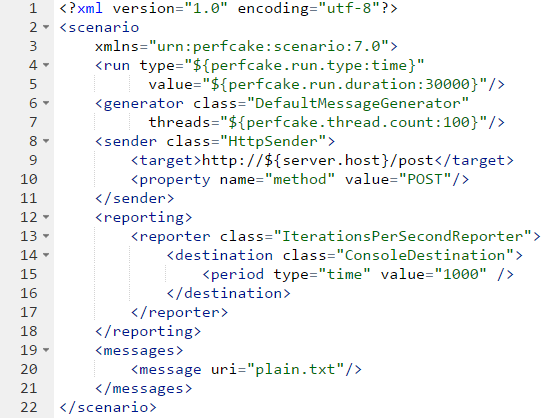
\includegraphics[scale=1]{scenario.png}
\caption{Scenár}\label{scenario}
\end{figure}


Pre jednoduchú ukážku si uvedieme príklad. Máme vyvinutý softvér, ktorý asynchrónne spracováva správy prichádzajúce pomocou POST metódy a HTTP protokolu. Následne tieto správy spracúva (validuje, vytvára záznamy do databázy, generuje reporty, ...) a po úspešnom spracovaní pošle potvrdzujúcu správu späť.
Na obrázku \ref{scenario} sa nachádza scenár pre jednoduchý testovací blok, ktorý by sme mohli na takýto nami vytvorený softvér použiť. Zo scenára je možné vidieť, že tento test bude bežať 3000 ms = 3 sekundy, generuje správy použitím 100 vlákien, ktoré posiela pomocou HTTP protokolu a metódy POST. Text správy je špecifikovaný v súbore``plain.txt'' a výsledky sú zaznamenávané na konzolu, každú 1 sekundu. Ako reporter je použitý ``IterationsPerSecondReporter'' a teda sa každú sekundu zapíše, koľko správ bolo softvérom spracovaných. Veľmi podobným scenárom by sme mohli testovať, koľko softvér používa pamäte, stačilo by zmeniť atribút reporter na ``MemoryUsageReporter''. Týmto spôsobom sa veľmi ľahko odhaľujú úniky pamäte. Scenáre sa púšťajú pomocou nástroja Maven alebo pomocou shell skriptu.


\section{Výstup}

Ako bolo uvedené v prvej podkapitole, Perfcake má viac možností východzích súborov. Okrem číselných výstupov má užívateľ tiež možnosť vykreslenia grafu.

\subsection{Dáta}
 Pri vytváraní algoritmu na optimalizáciu dát pre potreby vykresľovania do grafov, bude používaný formát súboru CSV.

\begin{table}[htb]
\centering
\begin{tabular}{|l|l|l|l|l|l|}
\hline
\multicolumn{3}{|c|}{\textit{\textbf{Throughput}}}  & \multicolumn{3}{c|}{\textit{\textbf{Memory}}}  \\ \hline
\textbf{Time} & \textbf{Current} & \textbf{Average} & \textbf{Time} & \textbf{Used} & \textbf{Total} \\ \hline
00:01:00      & 1,67             & 1,67             & 00:01:00      & 777,30        & 2817,06        \\ \hline
00:02:00      & 1,67             & 1,67             & 00:02:00      & 528,81        & 2835,94        \\ \hline
00:03:00      & 2,22             & 2,22             & 00:03:00      & 450,90        & 2901,19        \\ \hline
00:04:00      & 2,08             & 2,08             & 00:04:00      & 585,94        & 2911,63        \\ \hline
00:05:00      & 2,33             & 2,33             & 00:05:00      & 979,96        & 2953,00        \\ \hline
00:06:00      & 2,22             & 2,22             & 00:06:00      & 855,63        & 2960,25        \\ \hline
00:07:00      & 2,38             & 2,38             & 00:07:00      & 1193,20       & 2992,13        \\ \hline
00:08:00      & 2,29             & 2,29             & 00:08:00      & 1175,80       & 3001,75        \\ \hline
00:09:00      & 2,22             & 2,22             & 00:09:00      & 1197,66       & 3009,88        \\ \hline
00:10:00      & 2,17             & 2,17             & 00:10:00      & 831,64        & 3013,38        \\ \hline
00:11:00      & 2,27             & 2,27             & 00:11:00      & 1380,88       & 3019,63        \\ \hline
00:12:00      & 2,22             & 2,22             & 00:12:00      & 815,44        & 3031,56        \\ \hline
00:13:00      & 2,18             & 2,18             & 00:13:00      & 950,54        & 3035,38        \\ \hline
00:14:00      & 2,26             & 2,26             & 00:14:00      & 726,44        & 3036,44        \\ \hline
00:15:00      & 2,44             & 2,33             & 00:15:00      & 659,87        & 3042,88        \\ \hline
00:16:00      & 2,18             & 2,19             & 00:16:00      & 715,86        & 3042,88        \\ \hline
00:17:00      & 2,18             & 2,16             & 00:17:00      & 909,47        & 3042,44        \\ \hline
00:18:00      & 2,05             & 2,13             & 00:18:00      & 1016,83       & 3042,31        \\ \hline
00:19:00      & 2,14             & 2,19             & 00:19:00      & 697,72        & 3043,13        \\ \hline
00:20:00      & 2,05             & 2,17             & 00:20:00      & 844,43        & 3043,75        \\ \hline
\end{tabular}
\caption{Dáta}\label{tab:Data}
\end{table}

Tabuľka  \ref{tab:Data} ukazuje dáta vygenerované nástrojom Perfcake za 20 minút, testovala sa priepustnosť softvéru v iteráciách za sekundu a využitie pamäte v megabajtoch. Pri priepustnosti sa počíta priemer za časovú jednotku (current) a tiež priemer za niekoľko časových jednotiek (average), časová jednotka a veľkosť okna, s ktorými sa bude počíta sa 
dá nastaviť v scenári, pri dátach s tabuľky je to minúta a 15 záznamov. Priemer sa začína počítať, keď sa naplní okno a potom už pre každý ďalší záznam. 

\begin{figure}[!htb]
\centering
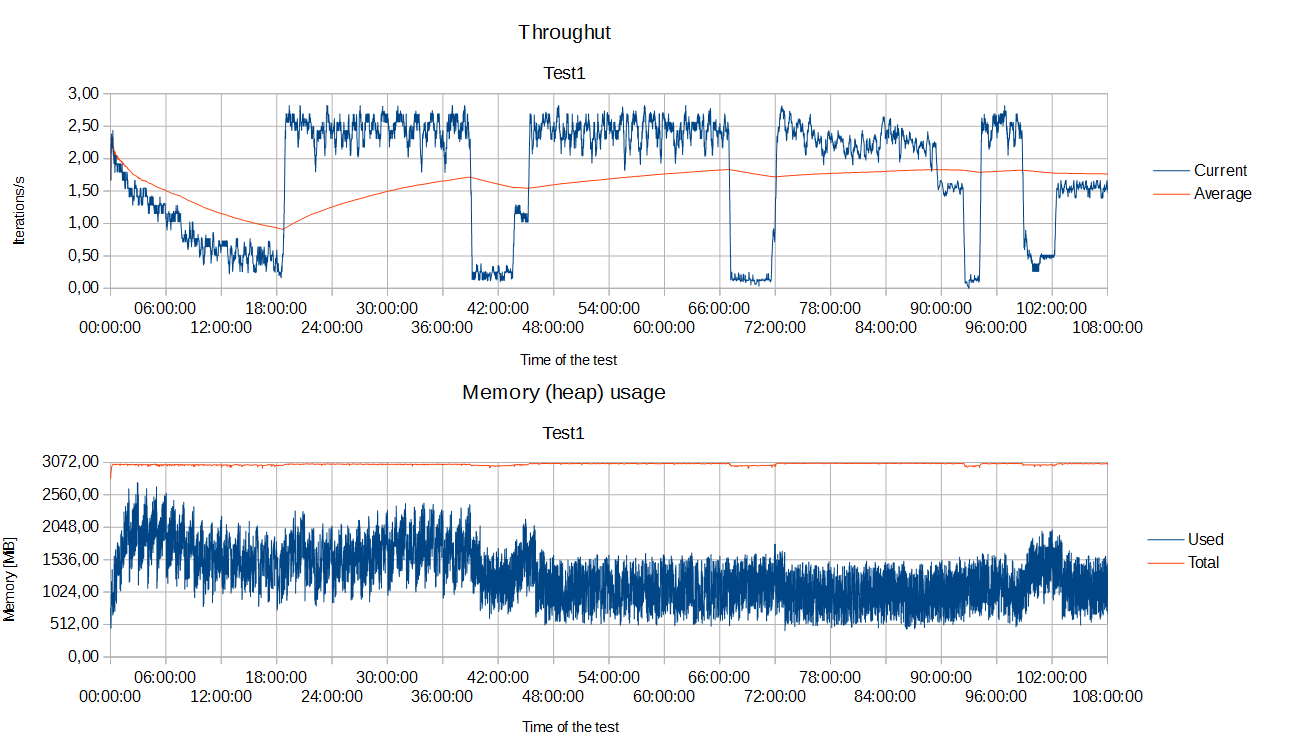
\includegraphics[scale=0.70, angle =90]{graphs.png}
\caption{Grafy}\label{grafy}
\end{figure}


Pri testovaní využívania pamäte sa zaznamenáva použitá (used) a celková pamäť (total). Celková pamäť, je pamäť, ktorú si  JVM alokuje a použitá pamäť je pamäť, ktorú naozaj využije - celková mínus voľná pamäť. Viac o pamäti v JVM sa čitateľ dozvie v oficiálnej dokumentácií(http://docs.oracle.com/javase/8/docs/api/java/lang/Runtime.html).

V popisovanej tabuľke sú dáta zaznamenané za 20 min, v praxi ale tie testy bežia väčšinou niekoľko desiatok hodín a teda tabuľky môžu dosahovať tisíce záznamov. Ukladať a následne spracovať takéto množstvo dát je pamäťovo aj časovo náročné a preto budem hľadať algoritmus, ktorý zmenší objem dát a zároveň neznehodnotí informáciu z nich vyplývajúcu, pri vykreslení do grafov.


\subsection{Grafy}

Pomocou grafu vieme často do mozgu preniesť oveľa viac informácií. 
Na obrázku  \ref{grafy} sú znázornené grafy z testov, ktoré bežali 108 hodín, a ktorých prvých 20 záznamov sme si ukázali v tabuľke  \ref{tab:Data}. Pre analýzu výsledku nie sú potrebné tak presné grafy, väčšinou je dôležitá hodnota okolo ktorej dáta v určitej časti grafu konvergujú, alebo či hodnoty veľmi ``skáču''. V bakalárskej práci budú tieto grafy upravené a následne porovnávané s grafmi, ktoré budú vykreslené z dát, na ktoré sa použije optimalizačný algoritmus.




%%%%%%%%%%%%%%%%%%%%%%%%%%%%%%%%%%%%
